\documentclass{article}
\usepackage{amsthm,amsmath,amsfonts,amssymb,mathtools}
\usepackage[colorlinks,citecolor=blue,urlcolor=blue]{hyperref}
\usepackage{enumitem}
\usepackage[margin=1in]{geometry}

% Some useful macros.
\newcommand{\given}{\,|\,}
\newcommand{\trans}{\mathsf{T}}
\newcommand{\bx}{\mathbf{x}}
\newcommand{\by}{\mathbf{y}}
\newcommand{\bw}{\mathbf{w}}
\newcommand{\distNorm}{\mathcal{N}}
\newcommand{\bzero}{\mathbf{0}}
\newcommand{\btheta}{\boldsymbol{\theta}}
\newcommand{\bpi}{\boldsymbol{\pi}}
\newcommand{\ep}{\varepsilon}
\def\ie{i.e.\ }
\def\eg{e.g.\ }
\def\iid{i.i.d.\ }
\def\simiid{\sim_{\mbox{\tiny iid}}}
\newcommand{\varv}{\mathbb{V}}
\newcommand{\LL}[1]{\frac{\partial \log \pi(a_{#1}| s_{#1}, \theta)}{\partial \theta}}
\newcommand{\PT}{\frac{\partial}{\partial \theta}}
\newcommand{\PP}[1]{\frac{\partial}{\partial #1}}
\newcommand{\PPH}{\frac{\partial}{\partial \phi}}
\newcommand{\LP}[1]{\PT \log p(#1)}
\newcommand{\LZ}[1]{\frac{\log \pi(z_{#1}| s_{#1}, \theta)}{\partial \theta}}
\newcommand{\N}{\mathcal{N}}

% for code
\usepackage{listings}
\usepackage{color}

\definecolor{string}{rgb}{0.561, 0.737, .7}
\definecolor{keyword}{rgb}{0.384,0.447,0.643}
\definecolor{comment}{rgb}{0.639,0.745,0.5}
%%
%% Julia definition (c) 2014 Jubobs
%%
\lstdefinelanguage{Julia}{
	morekeywords={
		abstract,break,case,catch,const,continue,do,else,elseif,end,export,false,for,function,immutable,import,importall,if,in,macro,module,otherwise,quote,return,switch,true,try,type,typealias,using,while
		},
	sensitive=true,
	morecomment=[l]\#,%
	morecomment=[n]{\#=}{=\#},%
	morestring=[s]{"}{"},
	morestring=[m]{'}{'},
}[keywords,comments,strings]

\lstset{
  language=Julia,
  aboveskip=3mm,
  belowskip=3mm,
  showstringspaces=false,
  columns=flexible,
  basicstyle={\small\ttfamily},
  numbers=none,
  numberstyle=\tiny\color{gray},
  keywordstyle=\color{keyword},
  commentstyle=\color{comment},
  stringstyle=\color{string},
  breaklines=true,
  breakatwhitespace=true,
  tabsize=4
}

% for graphics
\usepackage{graphicx}
\graphicspath{ {./plots/} }

\begin{document}
\title{Assignment 3: Variational Autoencoders}
\author{STA414/STA2014 and CSC412/CSC2506 Winter 2020\\
  David Duvenaud and Jesse Bettencourt\\
  Janet Wang 1003337980
}
\maketitle



\subsection{Background}
In this assignment, we will implement and investigate the Variational Autoencoder on binarized MNIST digits, as introduced by the paper \href{https://arxiv.org/pdf/1312.6114.pdf}{Auto-Encoding Variational Bayes} by Kingma and Welling (2013). Before starting, we recommend reading this paper.

\paragraph{Data.}
Each datapoint in the \href{http://yann.lecun.com/exdb/mnist/}{MNIST} dataset is a 28x28 grayscale image (i.e. pixels are values between 0 and 1) of a handwritten digit in $\{0 \dots 9\}$, and a label indicating which number.
MNIST is the `fruit fly' of machine learning -- a simple standard problem useful for comparing the properties of different algorithms.

Use the first 10000 samples for training, and the second 10000 for testing.
Hint: Also build a dataset of only 100 training samples to use when debugging, to make loading and training faster.

\paragraph{Tools.}
As before, you can (and should) use automatic differentiation provided by your package of choice.
Whereas in previous assignments you implemented neural network layers and stochastic gradient descent manually, in this assignment feel free to use those provided by a machine learning framework.
In Julia, these will be provided by \texttt{Flux.jl}.
You can also freely copy and adapt the Python autograd starter code provided.  
If you do, you should probably remove batch normalization.

However, you \textbf{may not use any probabilistic modelling elements} from these frameworks.
In particular, sampling from and evaluating densities under distributions must be written by you or provided by the starter code.


\subsection{Model Definition}

\paragraph{Prior.}
The prior over each digit's latent representation is a multivariate standard normal distribution.
For all questions, we'll set the dimension of the latent space $D_z$ to 2.
A larger latent dimension would provide a more powerful model, but for this assignment we'll use a two-dimensional latent space to make visualization and debugging easier..


\paragraph{Likelihood.}
Given the latent representation $z$ for an image, the distribution over all 784 pixels in the image is given by a product of independent Bernoullis, whose means are given by the output of a neural network $f_\theta(z)$:
$$p(x|z, \theta) = \prod_{d=1}^{784} \operatorname{Ber}(x_d|f_\theta(z)_d)$$
The neural network $f_\theta$ is called the decoder, and its parameters $\theta$ will be optimized to fit the data.


\pagebreak
\section{Implementing the Model [5 points]}

For your convenience we have provided the following functions:
\begin{itemize}
  \item \texttt{factorized\_gaussian\_log\_density} that accepts the mean and \textbf{log} standard deviations for a product of independent gaussian distribtuions and computes the likelihood under them. This function will produce the log-likelihood for each batch element $1 \times B$
  \item \texttt{bernoulli\_log\_density} that accepts the logits of a bernoulli distribution over $D$-dimensional data and returns $D \times B$ log-likelihoods.
  \item \texttt{sample\_diag\_gaaussian} that accepts above parameters for a factorized Gaussian distribution and samples with the reparameterization trick.
  \item \texttt{sample\_bernoulli} that accepts above parameters for a Bernoulli distribution and samples from it.
  \item \texttt{load\_binarized\_mnist} that loads and binarizes the MNIST dataset.
  \item \texttt{batch\_x} and \texttt{batch\_x} that splits the data, and just the images, into batches.
\end{itemize}

Further, in the file \texttt{example\_flux\_model.jl} we demonstrate how to specify neural network layers with Flux library.
Note that Flux provides convenience functions that allow us to take gradients of functions with respect to parameters that \textbf{are not passed around explicitly}.
Other AD frameworks, of if you prefer to implement your own network layers, recycling code from previous assignments, you may need to explicilty provide the network parameters to the functions below.

\begin{enumerate}[label=(\alph*)]
	% \item {\bf [2 points]} Load the MNIST dataset, and binarize the images.
	% That is, all the pixels with brightness more than 127 out of 255 should be set to 1, and all others set to 0.
	% Take the first 10000 images as a training set. %, and a separate test set of 10000 images.
	% Also, keep the image labels with the corresponding images.
	
  \item {\bf [1 point]} Implement a function \texttt{log\_prior} that computes the log of the prior over a digit's representation $\log p(z)$.
  
  \begin{lstlisting}
# log_prior: compute log of the prior over a digit's representation z
log_prior(z) = factorized_gaussian_log_density(0,0,z)
  \end{lstlisting}
	
  \item {\bf [2 points]} Implement a function \texttt{decoder} that, given a latent representation $z$ and a set of neural network parameters $\theta$ (again, implicitly in Flux), produces a 784-dimensional mean vector of a product of Bernoulli distributions, one for each pixel in a $28 \times 28$ image.
	Make the decoder architecture a multi-layer perceptron (i.e. a fully-connected neural network) with a single hidden layer with $500$ hidden units, and a \texttt{tanh} nonlinearity.
  Its input will be a batch two-dimensional latent vectors ($z$s in $D_z \times B$) and its output will be a 784-dimensional vector representing the logits of the Bernoulli means for each dimension $D_\text{data}\times B$.
	For numerical stability, instead of outputting the mean $\mu \in [0,1]$, you should output $\log \left( \frac{\mu}{1 - \mu} \right) \in \mathbb{R}$ called ``logit".
	
	% \item {\bf [3 points]} Implement a function \texttt{log\_prod\_Bernoulli} that, given an array of transformed Bernoulli mean parameters $\log \left( \frac{\mu}{1 - \mu} \right)$ and an equally-sized binary array $x$, computes the log-likelihood $\log \prod_d \operatorname{Ber}(x|\mu)$.
	% Hint: for numerical stability, you should use something like logaddexp to compute the Bernoulli log-probabilities.
	% It's easy to make a mistake here, so you might want to write a test for this function.

	\begin{lstlisting}
	## Model Dimensionality
	Dz, Dh = 2, 500
	Ddata = 28^2
	## Generative Model
	decoder = Chain(Dense(Dz, Dh, tanh), Dense(Dh, Ddata))
	\end{lstlisting}
	
	
	\item {\bf [1 point]} Implement a function \texttt{log\_likelihood} that, given a latent representation $z$ and a binarized digit $x$, computes the log-likelihood $\log p(x|z)$.
	
	\begin{lstlisting}
	### log_likelihood: given a latent representation $z$ and a binarized digit $x$,
	# computes the log-likelihood $\log p(x|z)$.
	function log_likelihood(x,z)
		""" Compute log likelihood log_p(x|z)"""
		# return likelihood for each element in batch
		p = decoder(z)
		# @info p, x
		return sum(bernoulli_log_density(p,x),dims=1)
	end
	\end{lstlisting}	
	
   	\item {\bf [1 point]} Implement a function \texttt{joint\_log\_density} which combines the log-prior and log-likelihood of the observations to give $\log p(z, x)$ for a single image.
	
	\begin{lstlisting}
	### joint_log_density: combines log-prior and log-likelihood of the observations
	# to give $\log p(z, x)$ for a single image. 
	joint_log_density(x,z) = log_prior(z) .+ log_likelihood(x,z)
	\end{lstlisting}

All of the functions in this section must be able to be evaluated in parallel, vectorized and non-mutating, on a batch of $B$ latent vectors and images, using the same parameters $\theta$ for each image.
In particular, you can not use a for loop over the batch elements.
  
\end{enumerate}

\pagebreak
\section{Amortized Approximate Inference and training [13 points]}
\begin{enumerate}[label=(\alph*)]
  	\item {\bf [2 points]} Write a function \texttt{encoder} that, given an image $x$ (or batch of images) and recognition parameters $\phi$, evaluates an MLP to outputs the mean and log-standard deviation of a factorized Gaussian of dimension $D_z = 2$.
	Make the encoder architecture a multi-layer perceptron (i.e. a fully-connected neural network) with a single hidden layer with $500$ hidden units, and a \texttt{tanh} nonlinearity.
	This function must be able to be evaluated in parallel on a batch of images, using the same parameters $\phi$ for each image.

	\begin{lstlisting}
	### encoder: evaluates MLP to give mean and log-standard deviation of a 
	# factorized Gaussian with Dim D_z=2.
	# MLP uses a single hidden layer with 500 hidden units and a tanh nonlinearity
	encoder = Chain(Dense(Ddata, Dh, tanh), Dense(Dh, Dz*2), unpack_gaussian_params)
	\end{lstlisting}

	\item {\bf [1 points]} Write a function \texttt{log\_q} that given the parameters of the variational distribution, evaluates the likelihood of $z$.
	
	\begin{lstlisting}
	### log_q: write log likelihood under variational distribution.
	log_q(q_mu, q_logsig, z) = factorized_gaussian_log_density(q_mu, q_logsig, z)
	\end{lstlisting}
	
	\item {\bf [5 points]} Implement a function \texttt{elbo} which computes an unbiased estimate of the mean variational evidence lower bound on a batch of images.
	Use the output of \texttt{encoder} to give the parameters for $q_\phi(z|\text{data})$.
	This estimator takes the following arguments:
	\begin{itemize}
		\item \texttt{x}, an batch of $B$ images, $D_x \times B$.
    	\item \texttt{encoder\_params}, the parameters $\phi$ of the encoder (recognition network). Note: these are not required with Flux as parameters are implicit.
		\item \texttt{decoder\_params}, the parameters $\theta$ of the decoder (likelihood). Note: these are not required with Flux as parameters are implicit.
	\end{itemize}
	This function should return a single scalar.
	Hint: You will need to use the reparamterization trick when sampling \texttt{zs}.
	You can use any form of the ELBO estimator you prefer.
  	(i.e., if you want you can write the KL divergence between q and the prior in closed form since they are both Gaussians).
	You only need to sample a single $z$ for each image in the batch.

	\begin{lstlisting}
	### elbo: computing unbiased estimate of the elbo on a batch of images xs
	function elbo(x)
		# variational parameters from data
		q_mu, q_logsigma = encoder(x) 
		# sample from variational distribution
		z = sample_diag_gaussian(q_mu, q_logsigma) 
		# joint likelihood of z and x under model
		joint_ll = joint_log_density(x,z)
		# likelihood of z under variational distribution 
		log_q_z = log_q(q_mu, q_logsigma, z)
		# Scalar value, mean variational evidence lower bound over batch
		elbo_estimate = mean(joint_ll - log_q_z, dims=2)
		return elbo_estimate[1]
	end
	\end{lstlisting}	
	
	\item {\bf [2 points]} Write a loss function called \texttt{loss} that returns the negative elbo estimate over a batch of data.
	
	\begin{lstlisting}
	### loss: gives negative elbo estimate over batch of data x
	function loss(x)
		# scalar value for the variational loss over elements in the batch
		return -elbo(x)
	end
	\end{lstlisting}
	
	
	\item {\bf [3 points]} Write a function that initializes and optimizes the encoder and decoder parameters jointly on the training set. 
    Note that this function should optimize with gradients on the elbo estimate over batches of data, not the entire dataset.
    Train the data for 100 epochs (each epoch involves a loop over every batch).
    Report the final ELBO on the test set.
	Tip: Save your trained weights here (e.g.\ with \texttt{BSON.jl}, see starter code, or by pickling in Python) so that you don't need to train them again.
	
	\begin{lstlisting}
	### train_model_params: initializes and optimizes the encoder and decoder params
	# jointly on the training set. Optimizes with gradients on the elbo estimate over 
	# batches of data, not the whole dataset. Trains for 10 epochs by default.
	# Training with gradient optimization:
	# See example_flux_model.jl for inspiration
	function train_model_params!(loss, encoder, decoder, train_x, test_x; nepochs=10)
		# model params: parameters to update with gradient descent
		ps = Flux.params(encoder, decoder)
		# ADAM optimizer with default parameters
		opt = ADAM()
		# over batches of the data
		for i in 1:nepochs
			for d in batch_x(train_x)
				# compute gradients with respect to variational loss over batch 
				# first argument is an anonymous function
				gs = Flux.gradient(() -> loss(d), ps) 
				# update the parameters with gradients
				Flux.Optimise.update!(opt, ps, gs)
			end
			if i%1 == 0 # change 1 to higher number to compute and print less frequently
				@info "Test loss at epoch $i: $(loss(batch_x(test_x)[1]))"
			end
		end
		@info "Parameters of encoder and decoder trained!"
	end
	\end{lstlisting}
	
\end{enumerate}

\pagebreak

\section{Visualizing Posteriors and Exploring the Model [15 points]}
In this section we will investigate our model by visualizing the distribution over data given by the generative model, sampling from it, and interpolating between digits.

\begin{enumerate}[label=(\alph*)]
	\item {\bf [5 points]} Plot samples from the trained generative model using ancestral sampling:	
	\begin{enumerate}[label=(\alph*)]

			\item First sample a z from the prior.
			\item Use the generative model to compute the bernoulli means over the pixels of $x$ given $z$. Plot these means as a greyscale image.
			\item Sample a binary image $x$ from this product of Bernoullis. Plot this sample as an image.
	\end{enumerate}
	Do this for 10 samples z from the prior.
	
	Concatenate all your plots into one 2x10 figure where each image in the first row shows the Bernoulli means of $p(x|z)$ for a separate sample of $z$, and each image in the the second row is a bianry image, sampled from the distribution above it.
	Make each column an independent sample.

	\begin{lstlisting}
		### 3a: plot samples from the trained generative model using ancestral sampling
		num_samples = 10
		
		# sample a z from the prior.
		sample_z = randn((2,num_samples))
		# compute the bernoulli means over the pixels of $x$ given $z$ using the generative model.
		bernoulli_means = 1.0 ./ (1.0 .+ exp.(-decoder(sample_z)))
		# Sample a binary image $x$ from this product of Bernoullis. Plot this sample as an image.
		binary_sample = sample_bernoulli(bernoulli_means)
		
		# plots of bernoulli means of p(x|z) for each sample of z
		plots_bernoulli = [plot(mnist_img(bernoulli_means[:,i]))  for i in 1:num_samples]
		# binary images sampled from the bernoulli distribution
		plots_binary =    [plot(mnist_img(binary_sample[:,i]))    for i in 1:num_samples]
		# each column is an independent sample
		plots = [ plots_bernoulli; plots_binary ]
		
		#### plot and save  3a
		display(plot(
			plots..., 
			layout = grid(2,num_samples), 
			size = (125*num_samples, 125*2)
		))
		savefig(joinpath("plots","3a.png"))
	\end{lstlisting}

	Final test set loss: 154.92761753905447
	Final ELBO on the test set: -154.87946244674814

	\begin{figure}[h]
		\centering
		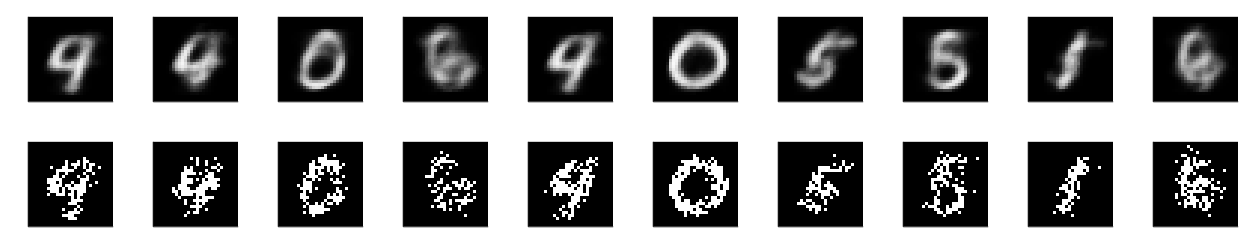
\includegraphics[width=\textwidth]{A3Q3a.png}
		\caption{Generative samples from the trained generative model using ancestral sampling. Top: Bernoulli means. Bottom: Binarized sample image.}
	  \end{figure}
	
	\item {\bf [5 points]} One way to understand the meaning of latent representations is to see which parts of the latent space correspond to which kinds of data.
	Here we'll produce a scatter plot in the latent space, where each point in the plot represents a different image in the training set.
	%will be the mean vector for the distribution $q_\phi(z|x)$ given by the encoder. Further, we will colour each point in the plot by the class label for the input data.
	
	\begin{enumerate}[label=(\alph*)]
		\item Encode each image in the training set.
		\item Take the 2D mean vector of each encoding $q_\phi(z|x)$.
		\item Plot these mean vectors in the 2D latent space with a scatterplot.
		\item Colour each point according to the class label (0 to 9).
	\end{enumerate}
	
	Hopefully our latent space will group images of different classes, even though we never provided class labels to the model!

	\begin{lstlisting}
	### 3b scatter plot where each point represents an image in the training set
	vector_x = [[] for i in 1:10]
	vector_y = [[] for i in 1:10]
	for i in 1:size(train_x)[2]
		# encode each image in the trianing set
		q_mu, q_logsigma = encoder(train_x[:,i]) 
		# take 2D mean vector of each encoding
		push!(vector_x[1 + train_label[i]], q_mu[1])
		push!(vector_y[1 + train_label[i]], q_mu[2])
	end

	#### plot and save 3b
	display(plot(
		vector_x,
		vector_y,
		seriestype = :scatter,
		title = "Latent Space Encoding from MNIST Training Set",
		xlabel = "z_1",
		ylabel = "z_2",
		label = ["0" "1" "2" "3" "4" "5" "6" "7" "8" "9"],
		size = (800, 800)
	))
	savefig(joinpath("plots","A3Q3b.png"))
	\end{lstlisting}

	See plot in Figure 2 at the end of the document.

	\begin{figure}[h]
		\centering
		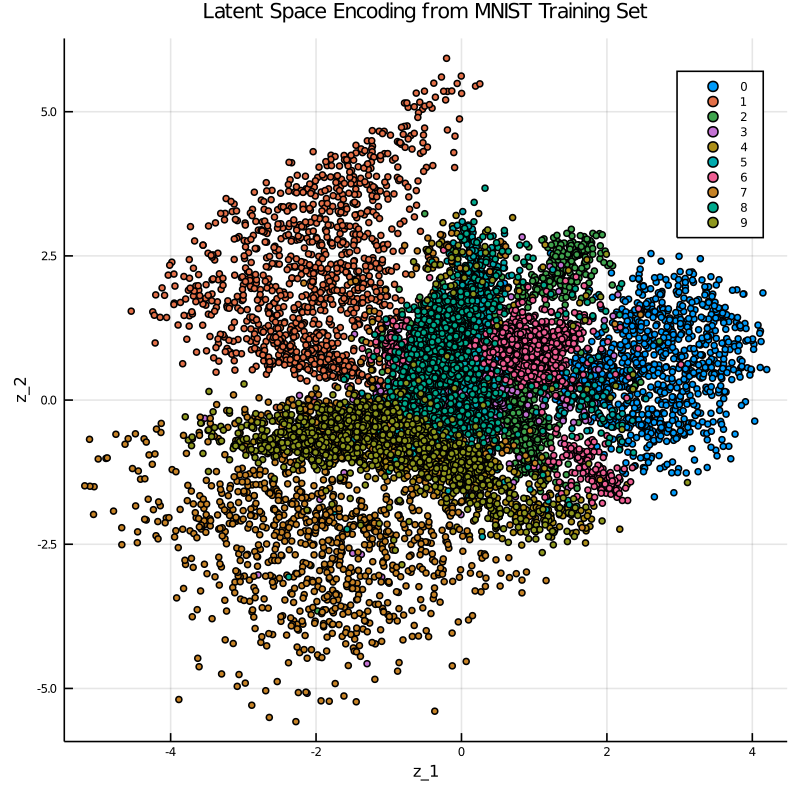
\includegraphics[width=\textwidth]{A3Q3b.png}
		\caption{Latent space encoding from MNIST training set}
	\end{figure}
	

	\item {\bf [5 points]} Another way to examine a latent variable model with continuous latent variables is to interpolate between the latent representations of two points.
	
	Here we will encode 3 pairs of data points with different classes. Then we will linearly interpolate between the mean vectors of their encodings. We will plot the generative distributions along the linear interpolation.
	
	\begin{enumerate}[label=(\alph*)]
		\item First, write a function which takes two points $z_a$ and $z_b$, and a value $\alpha \in [0,1]$, and outputs the linear interpolation $z_\alpha = \alpha z_a + (1 - \alpha) z_b$.
		\item Sample 3 pairs of images, each having a different class.
		\item Encode the data in each pair, and take the mean vectors
		\item Linearly interpolate between these mean vectors
		\item At 10 equally-space points along the interpolation, plot the Bernoulli means $p(x|z_\alpha)$
		\item Concatenate these plots into one figure.
	\end{enumerate}

	\begin{lstlisting}
		### 3c visualizing generative output along linear interpolations between mean
		# vectors of 3 pairs of encoded data points with different classes to examine 
		# the latent variable model

		# get linear interpolation of 2 points
		function linear_interpolation(za, zb, alpha)
			zalpha = alpha .* za + (1 - alpha) .* zb
			return zalpha
		end 

		# sample 3 pairs of images, each with a different class
		sample_images = [
			# 5, 0
			(train_x[:,1], train_x[:,2]),
			# 4, 1
			(train_x[:,3], train_x[:,4]),
			# 9, 2
			(train_x[:,5], train_x[:,5]),
		]

		# encode the data in each pair and take the mean vectors
		encoded_sample_images = [
			(encoder(sample_images[i][1]), encoder(sample_images[i][2])) 
			for i in 1:3
		]

		# make plots of the means at 10 equally spaced points
		plots = []
		for i in 1:3
			encoded_a, encoded_b = encoded_sample_images[i]
			for j in 1:10
					alpha = j/10.0
					meanalpha = linear_interpolation(encoded_a[1], encoded_b[1], alpha)
					# get Bernoulli means
					logit_mean = decoder(meanalpha)
					# plot means
					ber_mean = exp.(logit_mean) ./ (1 .+ exp.(logit_mean))
					push!(plots, plot(mnist_img(ber_mean[:])))
			end
		end

		#### plot and save
		display(plot(
			plots..., 
			layout=grid(3,10), 
			size =(850, 250),
			# layout=grid(10, 3), 
			# size =(500, 1700),
			axis = nothing
		))
		savefig(joinpath("plots","A3Q3c.png"))
	\end{lstlisting}

	See Figure 3 at the end of the document.

	\begin{figure}[h]
		\centering
		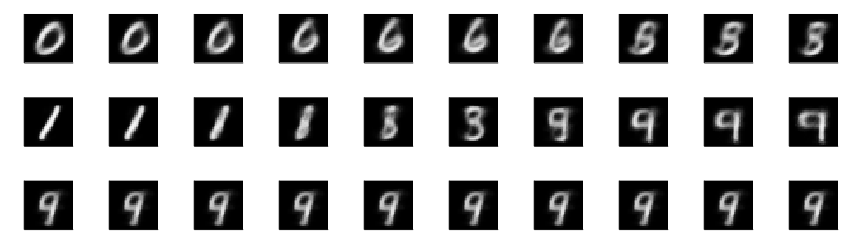
\includegraphics[width=\textwidth]{A3Q3c.png}
		\caption{Visualizing generative output along linear interpolations between mean vectors of 3 pairs of encoded data points with different classes}
	\end{figure}
	
\end{enumerate}


\pagebreak

\section{Predicting the Bottom of Images given the Top [15 points]}

Now we'll use the trained generative model to perform inference for $p(z|\text{top half of image x})$.
Unfortunately, we can't re-use our recognition network, since it can only input entire images.
However, we can still do approximate inference without the encoder.

To illustrate this, we'll approximately infer the distribution over the pixels in the bottom half an image conditioned on the top half of the image:
$$p(\text{bottom half of image x} | \text{top half of image x}) = \int p(\text{bottom half of image x} | z) p( z | \text{top half of image x}) dz$$
To approximate the posterior $p( z | \text{top half of image x})$, we'll use stochastic variational inference.

\begin{enumerate}[label=(\alph*)]	
	\item {\bf [5 points]} Write a function that computes $p(z, \text{top half of image x})$
	
	\begin{enumerate}[label=(\alph*)]
	\item First, write a function which returns only the top half of a 28x28 array. This will be useful for plotting, as well as selecting the correct Bernoulli parameters.
	
	\begin{lstlisting}
	#### top_half: gets top half of a 28x28 array
	function top_half(x)
		half_image = x[1:14*28, :]
		return half_image
	end
	\end{lstlisting}
	
    \item Write a function that computes $\log p(\text{top half of image x} | z)$. Hint: Given $z$, the likelihood factorizes, and all the unobserved dimensions of $x$ are leaf nodes, so can be integrated out exactly. 
	
	\begin{lstlisting}
	#### log_likelihood_top_half: computes log p(top half of image x| z)
	function log_likelihood_top_half(top_half_x, z)
		p = decoder(z)
		half_p = top_half(p)
		# sums top half
		sum(bernoulli_log_density(half_p, top_half_x), dims=1)
	end
	\end{lstlisting}
	
	\item Combine this likelihood with the prior to get a function that takes an x and an array of $z$s, and computes the log joint density $\log p(z, \text{top half of image x})$ for each $z$ in the array.
	
	\begin{lstlisting}
	#### joint_log_density_top_half: compute log p(z, top half of image x)
	# compute 3 log densities for the elbo: log p(z), log p(x|z), and log q(z).
	# log p(z) and log q(z) are both 2-dimensional Gaussians.
	joint_log_density_top_half(z, top_half_x) = 
		log_prior(z) .+ log_likelihood_top_half(top_half_x, z)
	\end{lstlisting}	

\end{enumerate}

	%\item {\bf [5 points]} Test your function by comparing the isocontours of $p(z | \text{top half of $x$})$ against the isocontours of $p(z | x)$.  Remember that these conditionals have the same isocontours as the joint distributions $p(z, \text{top half of $x$})$ and $p(z, x)$.  The 
	
	\item {\bf [5 points]} Now, to approximate $p(z | \text{top half of image x})$ in a scalable way, we'll use stochastic variational inference.  
    For a digit of your choosing from the training set (choose one that is modelled well, i.e. the resulting plot looks reasonable):

	\begin{enumerate}[label=(\alph*)]
		\item Initialize variational parameters $\phi_\mu$ and $\phi_{\log \sigma}$ for a variational distribution $q(z|\text{top half of $x$})$.
		
		\begin{lstlisting}
		phi_mu = randn(2, 10)
		phi_logsigma = randn(2, 10)
		\end{lstlisting}	
		
		\item Write a function that computes estimates the ELBO over $K$ samples $z \sim q(z|\text{top half of $x$})$.
		Use $\log p(z)$, $\log p(\text{top half of $x$} | z)$, and $\log q(z|\text{top half of $x$})$.
		
		\begin{lstlisting}
		#### elbo_svi: gets elbo over K samples $z -.- q(z|top half of x)$
		function elbo_svi(params, logp)
			# needs to be (2, k)
			phi_mu, p_logsigma = params
			# @info "elbo svi: $(size(phi_mu)) $(size(p_logsigma))"
			# needs to be (2, k)
			z = sample_diag_gaussian(phi_mu, p_logsigma)
			# @info "elbo svi samples z: $(size(z))"
			joint_ll = logp(z)
			# @info "joint_ll: $(size(joint_ll))"
			# likelihood of z under variational distribution 
			log_q_z = log_q(phi_mu, p_logsigma, z)
			# return sum(logp_estimate - logq_estimate) / k
			elbo_estimate = mean(joint_ll - log_q_z, dims=2)
			# Scalar value, mean variational evidence lower bound over batch
			# @info "elbo_estimate: $(elbo_estimate[1])"
			return elbo_estimate[1]
		end
		
		#### neg_elbo_svi: Takes parameters for q, evidence as an array of game outcomes,
		# and returns the -elbo estimate with k many samples from q
		function neg_elbo_svi(params; x = train_x) 
			# print(size(x))
			half_x = top_half(x)
			function logp(z)
				return joint_log_density_top_half(z, half_x)
			end
			return -elbo_svi(params, logp)
		end
		\end{lstlisting}	
		
		\item Optimize $\phi_\mu$ and $\phi_{\log \sigma}$ to maximize the ELBO.
		
		\begin{lstlisting}
		#### contours
		function contours!(f; colour=nothing)
			n = 100
			x = range(-1,stop=1,length=n)
			y = range(0,stop=1,length=n)
			z_grid = Iterators.product(x,y) # meshgrid for contour
			z_grid = reshape.(collect.(z_grid),:,1) # add single batch dim
			z = f.(z_grid)
			z = getindex.(z,1)'
			max_z = maximum(z)
			levels = [.99, 0.9, 0.8, 0.7, 0.6, 0.5, 0.4, 0.3, 0.2] .* max_z
			if colour==nothing
			p1 = contour!(x, y, z, fill=false, levels=levels)
			else
			p1 = contour!(x, y, z, fill=false, c=colour,levels=levels,colorbar=false)
			end
			plot!(p1)
		end
		
		### train_model_params_svi: optimize phi_mu and phi_logsigma 
		function train_model_params_svi!(init_params, data; num_itrs=200, lr= 1e-2)
			@info "Training model params using SVI"
			params_cur = init_params 
			for i in 1:num_itrs
				# gradients of variational objective with respect to parameters
				grad_params = gradient(
					params -> neg_elbo_svi(params, x = data), params_cur
				)[1]
				# update paramters with lr-sized step in descending gradient
				params_cur =  (
					params_cur[1] - lr * grad_params[1],
					params_cur[2] - lr * grad_params[2]
				)
				# report the current elbo during training
				if i%10 == 0 # change 1 to higher number to compute and print less frequently
					@info "Loss at iter $i: $(neg_elbo_svi(params_cur, x = data))"
			
					# plot true posterior in red and variational in blue
					# hint: call 'display' on final plot to make it display during training
					plot(
					title="Train model params using SVI: iteration $i");
					# plot likelihood contours for target posterior
					contours!(zs -> exp.(joint_log_density_top_half(zs, data)), colour=:red) 
					# display(skillcontour!(..., colour=:blue)) plot likelihood contours for variational posterior
					display(
					contours!(
						zs -> factorized_gaussian_log_density(params_cur[1], params_cur[2], zs), 
						colour=:blue
					)
					)
				end
			end
			return params_cur
		end
		\end{lstlisting}	
		
		\item On a single plot, show the isocontours of the joint distribution $p(z, \text{top half of image x})$, and the optimized approximate posterior $q_\phi(z | \text{top half of image x})$.
		
		\begin{lstlisting}
		### set up training model
		function set_up_svi(num_samples, x = train_x)
			train = x[:, 1:num_samples]
			half_train = top_half(train)
			phi_mu = randn(2, num_samples)
			phi_logsigma = randn(2, num_samples)
			return half_train, phi_mu, phi_logsigma
		end
		
		#### train the model
		half_train, phi_mu, phi_logsigma = set_up_svi(10000)
		params_svi = train_model_params_svi!((phi_mu, phi_logsigma), half_train; num_itrs=200, lr= 1e-2)
		\end{lstlisting}	

		See Figure 4 at end of document

		\begin{figure}[h]
			\centering
			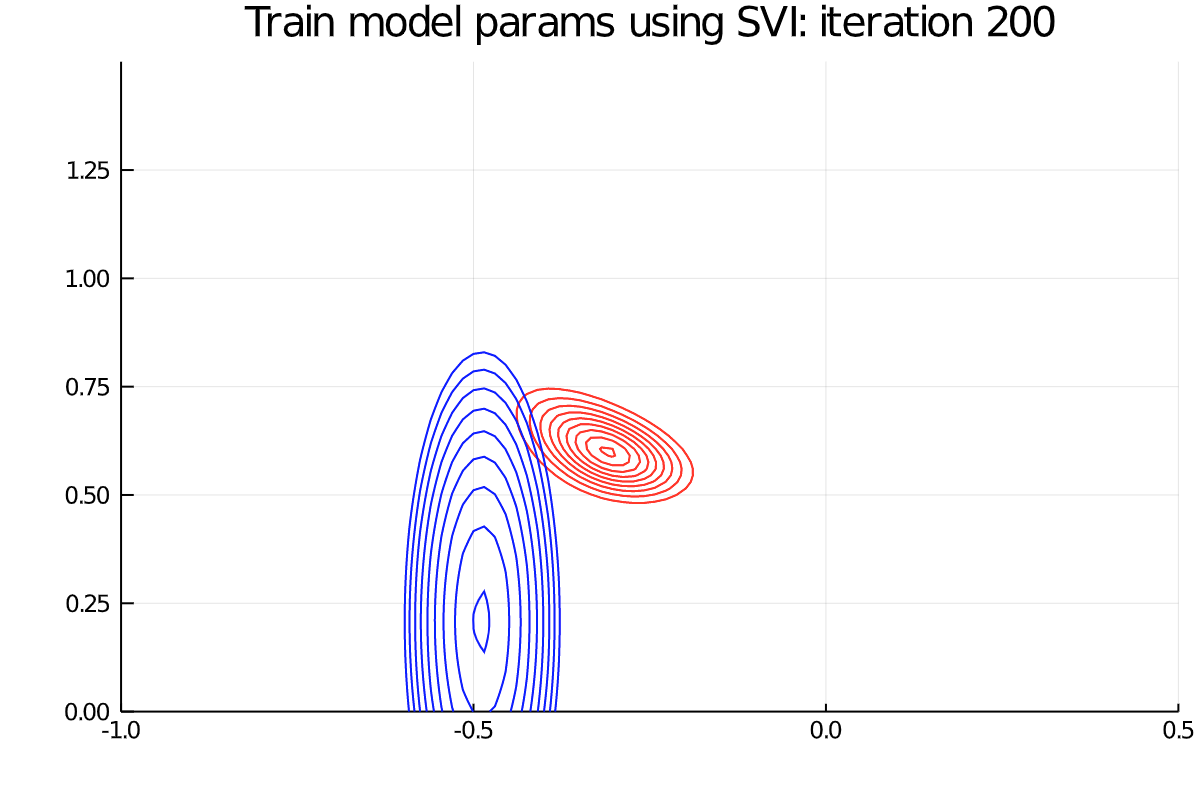
\includegraphics[width=\textwidth]{A3Q4bd.png}
			\caption{Isocontours of joint distribution (red) and optimized approximate posterior (blue)}
		\end{figure}
		
		\item Finally, take a sample $z$ from your approximate posterior, and feed it to the decoder to find the Bernoulli means of $p( \text{bottom half of image x}|z)$.  Contatenate this greyscale image to the true top of the image.
		Plot the original whole image beside it for comparison.
	
		\begin{lstlisting}
		# TODO
		\end{lstlisting}	
		
	\end{enumerate}

	\item {\bf [5 points]} True or false: Questions about the model and variational inference.
	
	There is no need to explain your work in this section.

\begin{enumerate}[label=(\alph*)]
	\item Does the distribution over $p(\text{bottom half of image $x$} | z)$ factorize over the pixels of the bottom half of image $x$?
	\\ Answer: Yes
	\item Does the distribution over $p(\text{bottom half of image $x$} | \text{top half of image $x$})$ factorize over the pixels of the bottom half of image $x$?
	\\ Answer: No
	\item When jointly optimizing the model parameters $\theta$ and variational parameters $\phi$, if the ELBO increases, has the KL divergence between the approximate posterior $q_\phi(z|x)$ and the true posterior $p_\theta(z|x)$ necessarily gotten smaller?
	\\ Answer: No
	\item If $p(x) = \mathcal{N}(x | \mu, \sigma^2)$, for some $x \in \mathbb{R}, \mu \in \mathbb{R}, \sigma \in \mathbb{R}^+$, can $p(x) < 0$?
	\\ Answer: False
	\item If $p(x) = \mathcal{N}(x | \mu, \sigma^2)$, for some $x \in \mathbb{R}, \mu \in \mathbb{R}, \sigma \in \mathbb{R}^+$, can $p(x) > 1$?
	\\ Answer: True
\end{enumerate}


\end{enumerate}



\end{document}
